\section{The shell}

\begin{frame}{What is a shell?}

\begin{block}{Shell}
Simply put, the shell is a program that takes commands from the keyboard and gives them to the operating system to perform\cite{whatIsTheShell}.
\end{block}

\begin{figure}
	\centering
	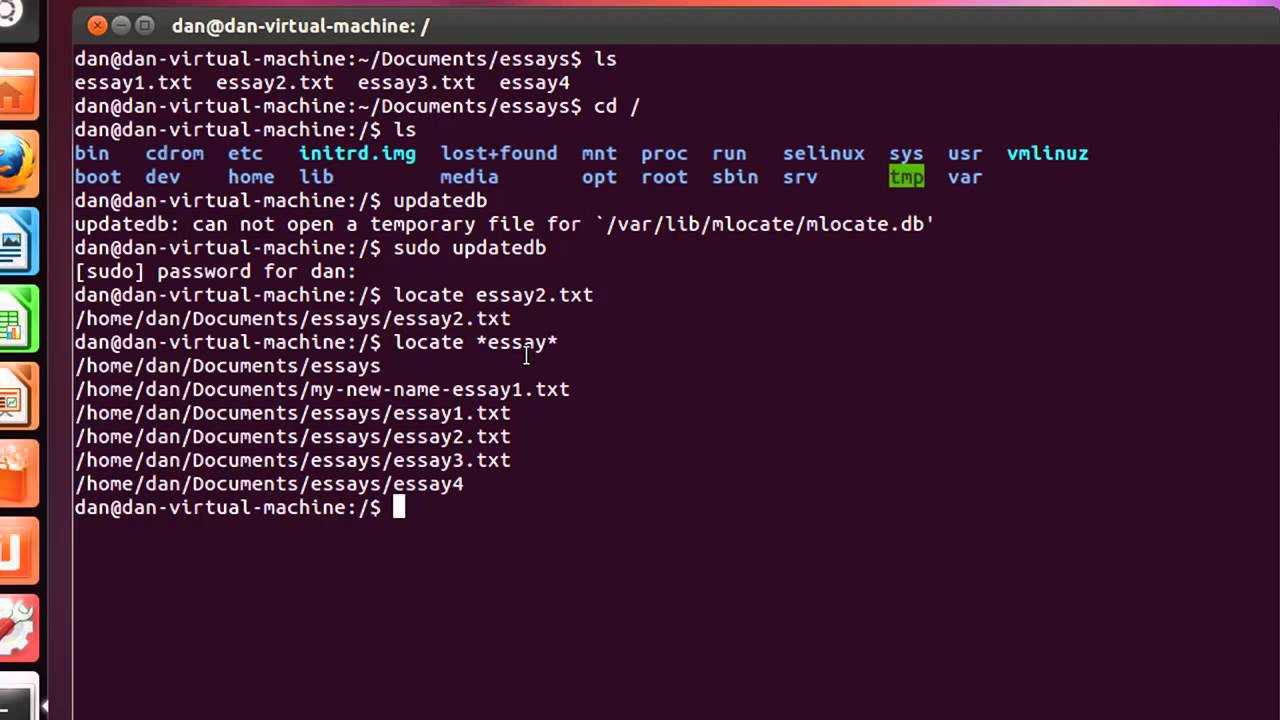
\includegraphics[width=1.0\textwidth]{terminal}
\end{figure}

\end{frame}

\begin{frame}{Shells implementations}
	A shell is an abstract concept. There are several implementations of a \code{shell}. Linux has different shells like \textit{bash}, \textit{sh}, \textit{ksh}. As for Windows, it has \textit{cmd} and \textit{power shell}.
	
	Each shell uses a different syntax for give commands ot the operating system. For instance:
	\begin{itemize}
		\item linux uses \code{ls -l} to print the files within a directory;
		\item windows uses \code{dir} to print the files within a directory;
	\end{itemize}
	
	Shells' syntaxes are theoretically different, but in reality they share lots fo similarities.
	
	\begin{note}
		We will show you \code{bash}, one of the most popular shells in linux.
	\end{note}
\end{frame}

\subsection{Bash: basic commands}

\begin{frame}{Open the shell}
	The shell has different names depending on your operating system. For example:
	\begin{itemize}
		\item Ubuntu: click on Unity bar (top icon on the left side) and type \mdQuote{terminal}. Click the icon to start the terminal \cite{ubuntu:openterminal};
		\item Gnome: \mdQuote{gnome-terminal};
		\item lxUbuntu: \mdQuote{lxterminal};
	\end{itemize}
	
	The shell will start in some directory in your system. For example is may start in \code{/home/your-username/};
\end{frame}

\begin{frame}{Really basic command}

	\begin{block}{man}
		\code{man} stands for \textbf{MANual}. If you want to know all the details about a command, invoke its manual. For example, if you want to know the details of \code{ls}, type \code{man ls}. Basically you type \code{man} followed by a space followed by the name of the command you want to read about. If you don't know the exact syntax of a command, be super sure to check its manual before asking questions! If people, after listening to a question of yours, reply with \mdQuote{RTFM}, it means you should have read the manual (RTFM stands for \mdQuote{\textbf{R}ead \textbf{T}he \textbf{F}unny/\textbf{F}*****g \textbf{M}anual}).
	\end{block}
	
\end{frame}

\begin{frame}{Command structure}
	Each command in \code{bash} has the following structure\cite{command:structure}:
	
	\begin{parcenter}[1pt]
		\texttt{command-name command-options command-arguments}
	\end{parcenter}	
	
	For example:
	
	\begin{parcenter}[1pt]
		\code{mkdir -p -v --mode=777 "hello/world"}
	\end{parcenter}
	
	\only<1>{
	\begin{enumerate}
		\item \code{command-name} is the name of the command, in this case \mdQuote{mkdir};
		\item \code{command options} area is an optional part of the command. It represents some flags, options that slightly alter the command behaviour. For example here the options are \mdQuote{-pv --mode=777}.
		\item \code{command arguments} (if any) represents the value the command mainly operate with. They are not prefixed by any \mdQuote{-} character whatsoever. For example \mdQuote{"hello/world"} represents the command arguments.
	\end{enumerate}
	}
	
	\only<2>{
		Options can be typed using 2 conventions: 
		\begin{itemize}
			\item \textbf{brief}(\code{-p}): Typically (but not always) \textit{brief} options have 1 \mdQuote{-} and one character. For example the command has 2 brief options, \code{-p} and \code{-v}. Brief options can be merged: for example typing \mdQuote{-p -v} is always equal (except in few instances) to \mdQuote{-pv}. 
			\item \textbf{long}(\code{--mode}): They are typically (but not always) prefixed by \mdQuote{--}. They are usually composed by more than one character (\ie \mdQuote{mode}).
		\end{itemize}
	}
	
	\only<3>{
		Both \textit{brief} and \textit{long} options can accept arguments. Normally it done using this syntax:
		\begin{itemize}
			\item \textbf{brief}: in general you type the character representing the option, a space and the value of the option (\ie{} \code{-m 777});
			\item \textbf{long}: in general you type the string of the option, a \mdQuote{=} and th value of the option(\ie{} \code{--mode=777});
		\end{itemize}
		
		\begin{note}
			Most options in most commands have both a \textit{brief} and a \textit{long} name. For instance, \mdQuote{-m} and \mdQuote{--mode} for \code{mkdir} commands are synonyms.
		\end{note}
	}
		
\end{frame}

\begin{frame}

	\begin{block}{pwd}
		\code{pwd} will return the \textbf{absolute path} of the directory you're currently in. Super useful if you got lost in the file system.
	\end{block}
	
	\begin{block}{ls}
		returns the list of files (and directories) in the directory you're in.
	\end{block}

\end{frame}



